\documentclass[12pt]{article}
\usepackage[a4paper]{geometry}
\usepackage[utf8]{inputenc}
\usepackage{fancyhdr}
\usepackage{lastpage}
\usepackage{graphicx, wrapfig, subcaption, setspace, booktabs}
\usepackage{graphicx}
\usepackage[T1]{fontenc}
\usepackage[font=small, labelfont=bf]{caption}
\usepackage[protrusion=true, expansion=true]{microtype}
\usepackage[english]{babel}
\usepackage{sectsty}
\usepackage{url, lipsum}
\usepackage[T1]{fontenc}
\usepackage{icomma}
\usepackage{siunitx}
\usepackage{ragged2e}
\usepackage{amsmath}
\usepackage{comment}
\usepackage{enumerate}
\usepackage{anysize}

\newcommand{\HRule}[1]{\rule{\linewidth}{#1}}
\onehalfspacing
\setcounter{tocdepth}{5}
\setcounter{secnumdepth}{5}

\begin{document}

\begin{titlepage}

\title{ \normalsize 
        \begin{center}
        
\includegraphics[height=6cm]{Logo.jpg}
        \end{center}
        \LARGE \textsc{\textbf{Universidad De Sonora}} \\ \bigskip
		\Large División de Ciencias Exactas y Naturales \\
        Licenciatura En Física \\ \bigskip
        \bigskip
        Física Computacional I
		\\ [0.1cm]  
		\HRule{2pt} \\
		\Large \textbf{{Reporte de Actividad 6}} \\
        \textit{\textbf{"Sistema de Resortes Acoplados"}}
		\HRule{2pt} \\
		\normalsize \vspace*{0.001\baselineskip}}
        
\date{\bigskip \Large Hermosillo, Sonora  \hspace*{\fill}  Marzo 19 de 2018}

        
\author{
		\Large\textbf{ César Omar Ramírez Álvarez} \\ \bigskip
        \\ \bigskip
       \Large Profr. Carlos Lizárraga Celaya}
       \end{titlepage}
       \maketitle
       

\newpage
\pagestyle{plain}

\section*{Introdución}
El presente informe es producto de la sexta práctica de la materia Física Computacional I, la cual tiene como objetivo aprender a modelar un fenómeno físico, en esta ocasión tomando de ejemplo un sistema de doble resorte acoplado, a través de una simulación.\\

Como es el caso de actividades anteriores, iniciaremos mostrando una breve síntesis sobre la teoría que hay detrás de nuestro sistema físico, basándonos en el artículo “Coupled Spring Equations” de los autores Fay y Graham. A diferencia de actividades anteriores que se trabajaba el código en Python mediante Jupyter Notebook, esta vez, exploramos a Jupyter Lab, un entorno que nos muestra un poco más de herramientas para Python. Presentaremos el código utilizado para resolver los diferentes problemas de una manera numérica con la ayuda de la biblioteca scipy.integrate.odeint, además mostraremos el error relativo existente entre lo calculado mediante el código y la solución analítica dada por el artículo. Visualizaremos una serie de gráficas generadas con los datos y finalizaremos con una conclusión general acerca de lo que fue la práctica mostrando reflexiones de lo aprendido en ella.

\section*{Síntesis}
La perspectiva general con la que se toma a las ecuaciones diferenciales esta cambiando mucho, de realizar técnicas para encontrar soluciones analíticas a visualizar y resolver numéricamente éstas con las herramientas disponibles.\\

En este artículo, se investiga uno de los problemas mas interesantes de la Mecánica, y que ahora normalmente se utiliza para la introducción al estudio de ecuaciones diferenciales. Este problema es el de los dos resortes con dos masas conectadas en serie, colgando del techo. Si suponemos que las fuerzas restauradoras de los resortes obedecen la Ley de Hooke, estos dos grados de libertad nos dan un modelo de ecuaciones diferenciales lineales de segundo grado. Al sustituir una ecuación en la otra, el movimiento de las masas puede ser descrito por una ecuación diferencial lineal de cuarto grado.\\

Con estas ecuaciones, podemos investigar los movimientos de las dos masas, para saber si están sincronizadas o si son opuestas. Además, hacer esto permite tener una interpretación física clara de la fase, amplitud, periodicidad, y la sensibilidad del sistema a las condiciones iniciales cuando se introduce la no linealidad.

\subsection*{El Modelo de los Resortes Acoplados}
\begin{wrapfigure}{r}{0.39\textwidth}
    \centering
    \includegraphics[width=0.213\textwidth]{resortes.png}
\end{wrapfigure}
El modelo consiste en dos resortes y dos masas. Un resorte con una constante $k_1$, está colgado del techo con una masa $m_1$ colgando de él.
De aquí, se cuelga otro resorte con una constante $k_2$ y debajo de él colgando una masa $m_2$. Al tenerlos en reposo, los resortes se estiran una distancia, a la que nombramos $x_1$ y $x_2$.

\subsection*{Asumiendo la Ley de Hooke}
Asumiendo que el sistema se mueve con oscilaciones pequeñas, podemos asumir que los resortes tendrán una fuerza restauradora dada por la Ley de Hooke, de la forma: $-k_1$$l_1$ y $-k_2$$l_2$ donde $l_1$ y $l_2$ son las elongaciones o comprensiones de los resortes. Como $m_1$ está atada a los dos resortes, en ella actúan las dos fuerzas restauradoras, mientras que $m_2$ solamente “siente” la fuerza restauradora del segundo resorte. Sin fricción, la Segunda Ley de Newton para estas dos masas es:\\
\centerline{$m_1 \ddot x_1 = -k_1x_1 - k_2(x_1-x_2)$}
\centerline{$m_2 \ddot x_2 = -k_2(x_2-x_1)$}\\

Para encontrar una ecuación para $x_1$ que no involucre a $x_2$, resolvemos la ecuación de $x_2$, y sustituyendo esta ecuación en las ecuaciones anteriores se llega a la siguiente ecuación diferencial de cuarto grado:\\
\centerline{$m_1m_2x_1^{(4)} + (m_2k_1 + k_2(m_1+m_2)) \ddot x_1 + k_1k_2x_1=0$}\\

Haciendo este mismo proceso, pero para $x_2$, se llega a la misma ecuación anterior. Es necesario solamente las posiciones y velocidades para poder determinar la solución.

\subsection*{Ejemplos con Masas Idénticas}
\textbf{\textit{2.1 Describe el movimiento para un sistema de resortes con $k_1$$=6$ y $k_2$$=4$ con condiciones iniciales de $(x_1(0), \dot x_1(0), x_2(0), \dot x_2(0))=(1,0,2,0)$.}}\\

Resolviendo el problema de una forma analítica, se llega a que las ecuaciones para las posiciones de las masas son:\\
\centerline{$x_1(t)=cos\sqrt2t$}
\centerline{$x_2(t)=2cos\sqrt2t$}\\

A continuación, se presenta la sección de código utilizada para encontrar numéricamente los resultados con Python en Jupyter Lab. (La primera imagen es la misma para los primeros 4 ejemplos).
\begin{center}
	\includegraphics[height=6cm]{2_1a.png}
\end{center}
\begin{center}
    \includegraphics[height=14cm]{2_1b.png}
\end{center}
\begin{center}
    \includegraphics[height=3.5cm]{2_1c.png}\hspace*{\fill}
    \includegraphics[height=2.5cm]{2_1d.png}
\end{center}
\begin{center}
    \includegraphics[height=2.5cm]{2_1e.png}\hspace*{\fill}
    \includegraphics[height=2.5cm]{2_1f.png}
\end{center}
Las gráficas que se obtuvieron son:
\begin{center}
    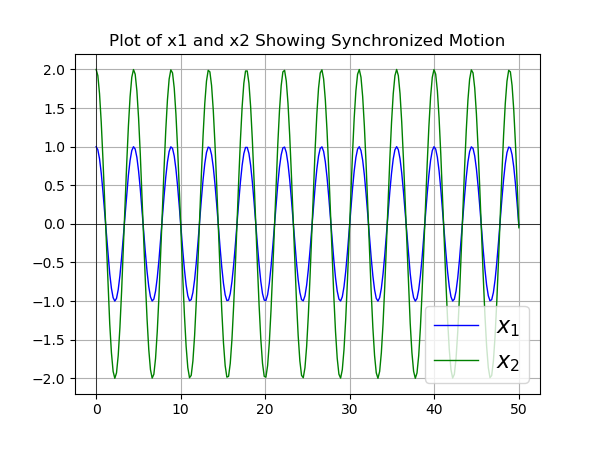
\includegraphics[height=6cm]{G2_1a.png}\hspace*{\fill}
    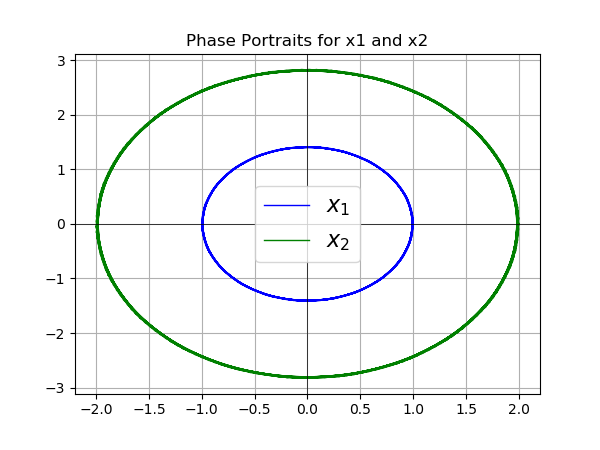
\includegraphics[height=6cm]{G2_1b.png}\\
    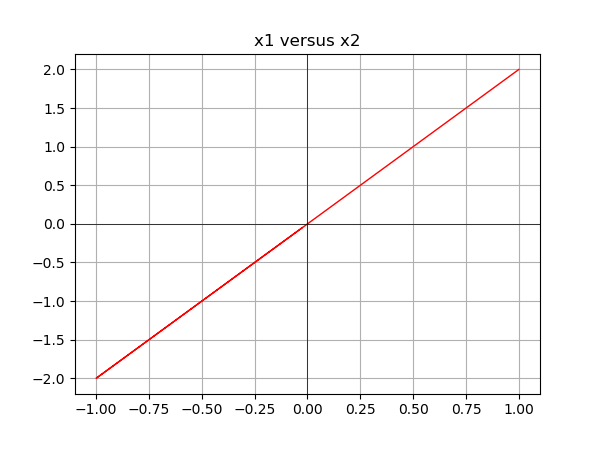
\includegraphics[height=6cm]{G2_1c.png}\
\end{center}
Describiendo lo anterior, podríamos decir que tenemos un movimiento que esta sincronizado, ya que, aunque se tienen amplitudes diferentes, las masas se mueven en fase una con la otra lo cual es notorio en la primera gráfica. Las elipses de la segunda gráfica muestran la variación de la amplitud y al graficar las posiciones una contra la otra nos genera una línea recta notable en la tercera gráfica.\\

\textbf{\textit{2.2 Describe el movimiento para un sistema de resortes con $k_1$$=6$ y $k_2$$=4$ con condiciones iniciales de $(x_1(0), \dot x_1(0), x_2(0), \dot x_2(0))=(-2,0,1,0)$.}}\\

La solución analítica es:\\
\centerline{$x_1(t)=-2cos2\sqrt3t$}
\centerline{$x_2(t)=cos2\sqrt3t$}\\

A continuación, se presenta la sección de código utilizada para encontrar numéricamente los resultados con Python en Jupyter Lab.

\begin{center}
    \includegraphics[height=14cm]{2_2a.png}
\end{center}
\begin{center}
    \includegraphics[height=4.5cm]{2_2b.png}
\end{center}
\begin{center}
    \includegraphics[height=2.5cm]{2_2c.png}\hspace*{\fill}
    \includegraphics[height=2.5cm]{2_2d.png}\\
\end{center}
Las gráficas que se obtuvieron son:
\begin{center}
    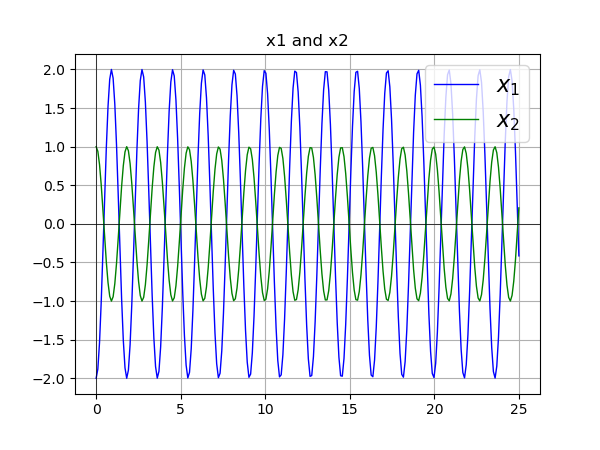
\includegraphics[height=6cm]{G2_2a.png}\hspace*{\fill}
    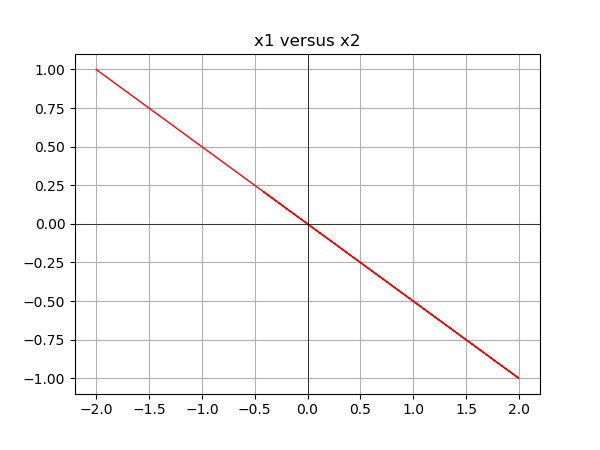
\includegraphics[height=6cm]{G2_2b.png}\\
\end{center}
En este caso, la primera masa se mueve hacia abajo mientras que la segunda se mueve hacia arriba, con el mismo periodo, pero en desfase.\\

\textbf{\textit{2.3 Describe el movimiento para un sistema de resortes con $k_1$$=0.4$ y $k_2$$=1.808$ con condiciones iniciales de $(x_1(0), \dot x_1(0), x_2(0), \dot x_2(0))=(1/2,0,-1/2,7/10)$.}}\\

A continuación, se presenta la sección de código utilizada para encontrar numéricamente los resultados con Python en Jupyter Lab.
\begin{center}
    \includegraphics[height=14cm]{2_3a.png}
\end{center}
\begin{center}
    \includegraphics[height=4.5cm]{2_3b.png}
\end{center}
\begin{center}
    \includegraphics[height=2.5cm]{2_3c.png}\hspace*{\fill}
    \includegraphics[height=2.5cm]{2_3d.png}\\
\end{center}
\begin{center}
    \includegraphics[height=3cm]{2_3e.png}\hspace*{\fill}
    \includegraphics[height=3cm]{2_3f.png}\\
\end{center}
\begin{center}
    \includegraphics[height=3cm]{2_3g.png}\hspace*{\fill}
    \includegraphics[height=2.5cm]{2_3h.png}\\
\end{center}
Las gráficas que se obtuvieron son:
\begin{center}
    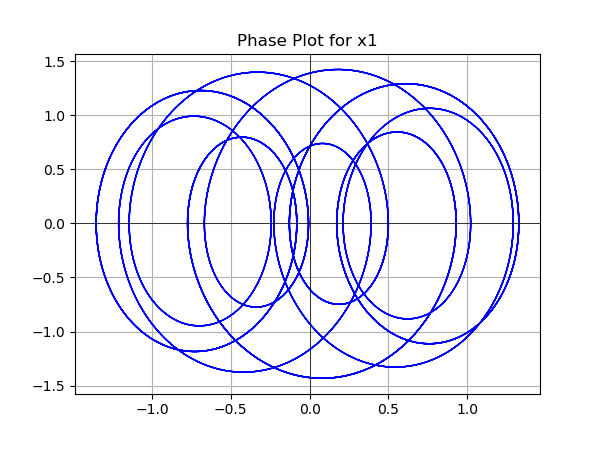
\includegraphics[height=6cm]{G2_3a.png}\hspace*{\fill}
    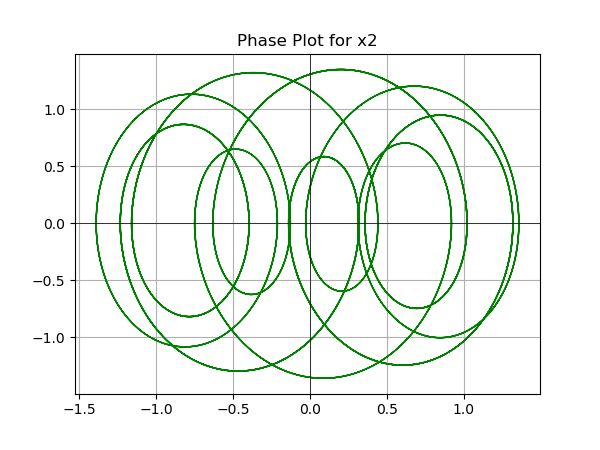
\includegraphics[height=6cm]{G2_3b.png}\\
    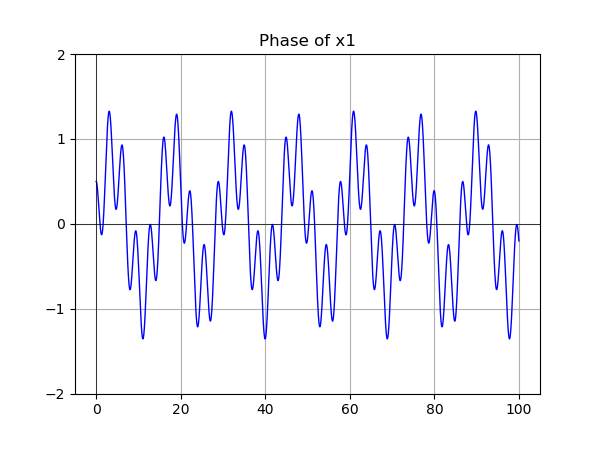
\includegraphics[height=6cm]{G2_3c.png}\hspace*{\fill}
    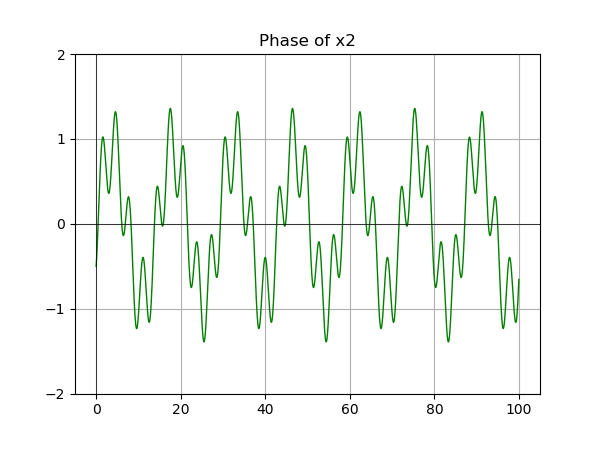
\includegraphics[height=6cm]{G2_3d.png}\\
    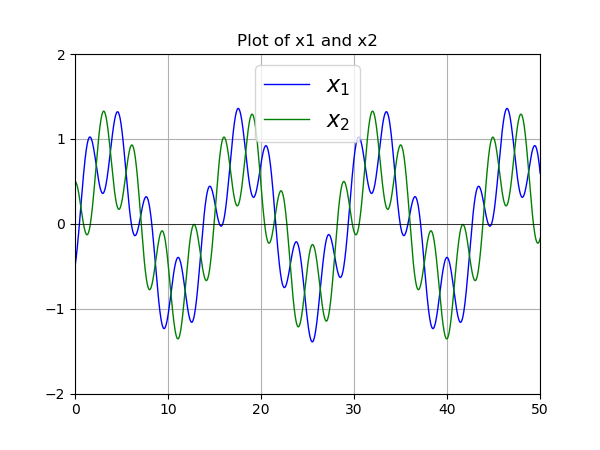
\includegraphics[height=6cm]{G2_3e.png}\hspace*{\fill}
    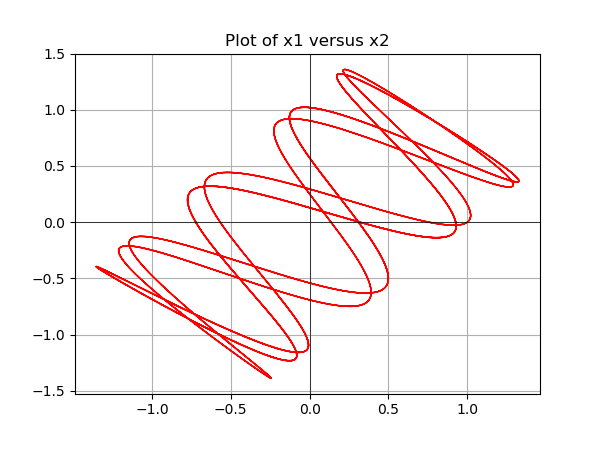
\includegraphics[height=6cm]{G2_3f.png}\\
\end{center}
Es notorio en la observación de los resultados que las condiciones iniciales solo afectan a la amplitud y a la fase de las soluciones, mientras que las constantes de cada uno de los resortes influyen en la determinación de la frecuencia y el fenómeno del sistema.
\subsection*{Amortiguamiento}
Los problemas más generales acerca de amortiguamiento es el de viscosidad, en donde la fuerza de amortiguamiento es proporcional a la velocidad. El amortiguamiento de la primera masa depende solamente de su velocidad y no en la de la segunda y viceversa. Asumimos que
los coeficientes de amortiguamiento $\delta_1$ y $\delta_2$ son pequeños. El modelo se convierte y descrito por lo siguiente:\\
\centerline{$m_1 \ddot x_1 = -\delta_1 \dot x_1 -k_1x_1 - k_2(x_1-x_2)$}
\centerline{$m_2 \ddot x_2 = -\delta_2 \dot x_2 -k_2(x_2-x_1)$}\\

Para obtener la ecuación de movimiento para una de las variables de posición ($x_1$ o $x_2$) se realiza el mismo procedimiento que en la sección anterior, es decir, se sustituye en una ecuación en la ecuación anterior que le corresponde, así se obtiene una nueva ecuación diferencial de cuarto grado para ambas posiciones de $x$.\\

\textit{\textbf{2.4 Asumiendo que $m_1$$=m_2$$=1$. Describe el movimiento para un sistema de resortes con $k_1$$=0.4$ y $k_2$$=1.808$, con coeficientes de amortiguamiento $\delta_1$$=0.1$ y $\delta_2$$=0.2$ con condiciones iniciales de $(x_1(0), \dot x_1(0), x_2(0), \dot x_2(0))=(1,1/2,2,1/2)$.}}\\

A continuación, se presenta la sección de código utilizada para encontrar numéricamente los resultados con Python en Jupyter Lab.
\begin{center}
    \includegraphics[height=14cm]{2_4a.png}
\end{center}
\begin{center}
    \includegraphics[height=4.5cm]{2_4b.png}
\end{center}
\begin{center}
    \includegraphics[height=3cm]{2_4c.png}\hspace*{\fill}
    \includegraphics[height=3cm]{2_4d.png}\\
\end{center}
\begin{center}
    \includegraphics[height=3cm]{2_4e.png}\hspace*{\fill}
    \includegraphics[height=3cm]{2_4f.png}\\
\end{center}
\begin{center}
    \includegraphics[height=3cm]{2_4g.png}\hspace*{\fill}
    \includegraphics[height=2.7cm]{2_4h.png}\\
\end{center}
Las gráficas que se obtuvieron son:
\begin{center}
    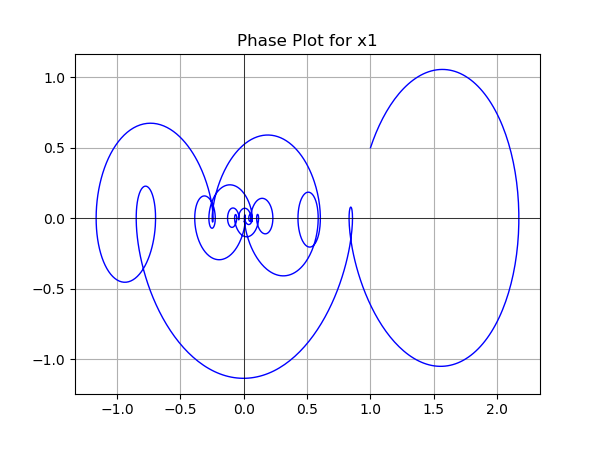
\includegraphics[height=6cm]{G2_4a.png}\hspace*{\fill}
    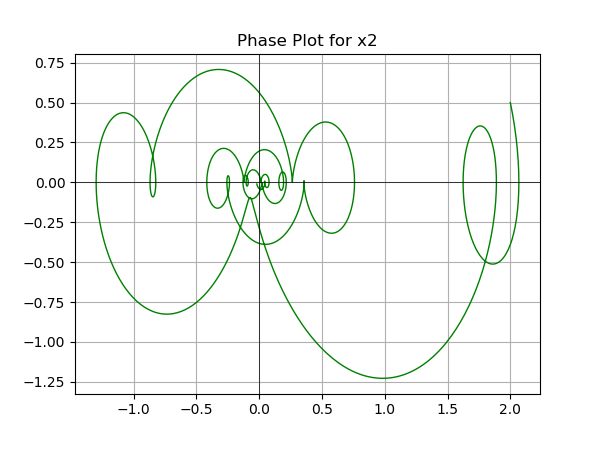
\includegraphics[height=6cm]{G2_4b.png}\\
    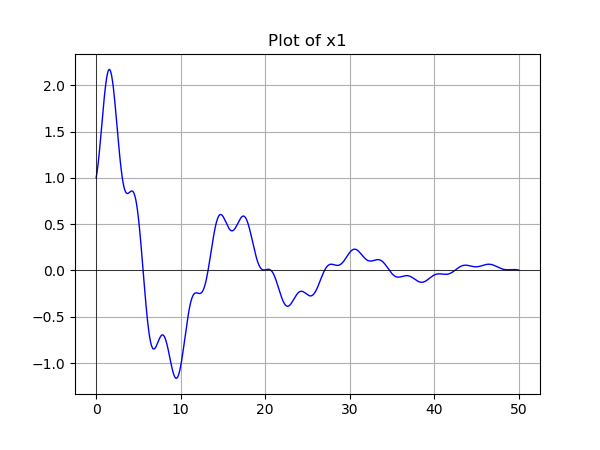
\includegraphics[height=6cm]{G2_4c.png}\hspace*{\fill}
    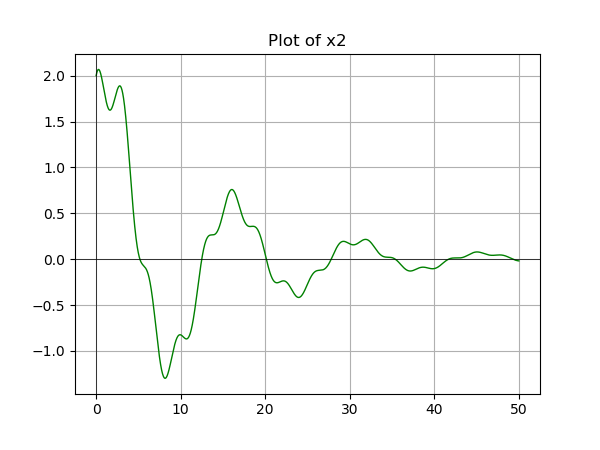
\includegraphics[height=6cm]{G2_4d.png}\\
    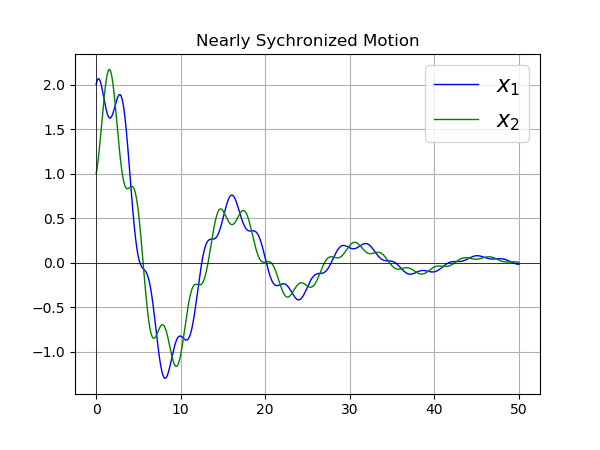
\includegraphics[height=6cm]{G2_4e.png}\hspace*{\fill}
    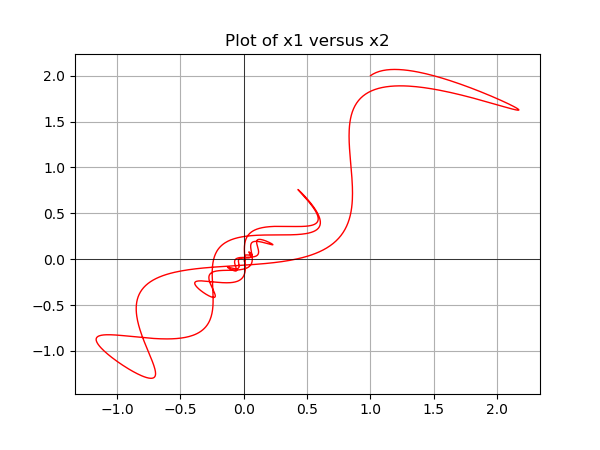
\includegraphics[height=6cm]{G2_4f.png}\\
\end{center}
De lo anterior es rescatable que, ahora existiendo amortiguamiento, las amplitudes disminuyen conforme el paso del tiempo. Se puede observar cierta sincronia al graficar $x_1$ y $x_2$, a pesar de que tienen distintas condiciones iniciales.

\subsection*{Solución Análitica y Solución Numérica}
Contando con los dos tipos de soluciones: porporcionada por Python (numérica) y porporcionada por el artículo (analítica) es posible realizar el calculo del error relativo. Esto se hace mediante el valor real y nuestra aproximación obtenida. En los archivos creados en los ejercicios 2.1 y 2.2 se imprimió el error relativo, calculado de la siguiente manera: restando el valor real al aproximado dividiendo lo anterior entre el valor real.\\
El código para gráficar el error fue el siguiente:
\begin{center}
    \includegraphics[height=2.5cm]{2_1g.png}\hspace*{\fill}
    \includegraphics[height=2.5cm]{2_1h.png}\\
\end{center}
\begin{center}
    \includegraphics[height=2.5cm]{2_2e.png}\hspace*{\fill}
    \includegraphics[height=2.6cm]{2_2f.png}\\
\end{center}
Mientras que las gráficas son:
\begin{center}
    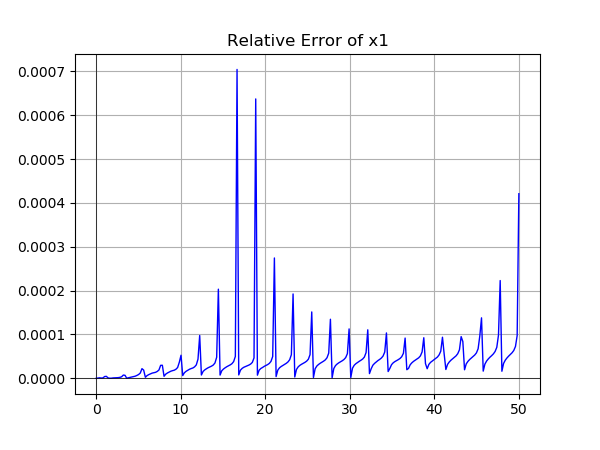
\includegraphics[height=6cm]{G2_1d.png}\hspace*{\fill}
    \includegraphics[height=6cm]{G2_1e.png}\\
    \includegraphics[height=6cm]{G2_2c.png}\hspace*{\fill}
    \includegraphics[height=6cm]{G2_2d.png}\\
\end{center}
Podemos decir que para ambos ejemplos los errores son muy pequeños y muy idénticos entre $x_1$ y $x_2$. 

\section*{Conclusión}
Jupyter Lab como entorno de trabajo, me parecio una mas eficaz que cuando haciamos uso de Jupyter Notebook, pues en este nuevo entorno se pueden realizar más cosas y tener un control de lo que estamos generando con el código. Además con el uso de la biblioteca para integrar fue posible resolver de manera muy rápida las ecuaciones diferenciales propuestas en los ejercicios.\\

El tema fue bastante interesante, creo que fue muy buena ejemplificación para el uso de las nuevas herramientas y conocimientos alcanzados, ya que, es un tema común en la Licenciatura que se aborda como estudio en materias como Mecánica y es bueno tener un repaso y conocimiento del mismo tanto de manera teórica como analítica. Sin duda Python es muy habil para hacer lectura de archivos y realizar calculos numéricos con los mismos.

\section*{Bibliografía}
\begin{itemize}
\item Integration and ODEs (scipy.integrate) — SciPy v1.0.0 Reference Guide. (2018). Docs.scipy.org. Recuperado el 12 de Marzo de 2018 desde\\
https://docs.scipy.org/doc/scipy/reference/integrate.html
\item  JupyterLab Documentation — JupyterLab 1.0 Beta documentation. (2018). Jupyterlab.readthedocs.io.  Recuperado el 12 de Marzo de 2018 desde \\
http://jupyterlab.readthedocs.io/en/latest/
\item Coupled spring-mass system — SciPy Cookbook documentation. (2018). Scipy-cookbook.readthedocs.io. Recuperado el 12 de Marzo de 2018 desde\\
http://scipy-cookbook.readthedocs.io/items/CoupledSpringMassSystem.html
\end{itemize}

\section*{Apéndice}
\begin{enumerate}
\item ¿En general te pareció interesante esta actividad de modelación matemática? ¿Qué te gustó mas? ¿Qué no te gustó?\\
\textit{Me pareció bastante interesante el tema y las gráficas que se generaban con los datos, pero siento que le faltaron un poco más de referencia y explicación a lo que se iba a realizar.}

\item La cantidad de material te pareció ¿bien?, ¿suficiente?, ¿demasiado?\\
\textit{Fue lo suficiente, aunque parecia mucha en un principio.}

\item ¿Cuál es tu primera impresión de Jupyter Lab? \\
\textit{A diferencia de Notebook, me parecio más fácial de entender y con un mejor diseño, además cuenta con mejores herramientas.}

\item Respecto al uso de funciones de SciPy, ¿ya habías visto integración numérica en tus cursos anteriores? ¿Cuál es tu experiencia?.\\
\textit{Si eh visto, en Programación y Análisis Numérico pero en FORTRAN con Trapecios y Simpson.}

\item El tema de sistema de masas acopladas con resortes, ¿ya lo habías resuelto en tu curso de Mecánica 2?  \\
\textit{Si, pero sin tantas condiciones fue explicación sencilla.}

\item ¿Qué le quitarías o agregarías a esta actividad para hacerla más interesante y divertida? \\
\textit{Sugiero mas referencias y explicación de lo que vamos a realizar, a veces me pierdo.}
\end{enumerate}






\end{document}
